\uuid{xpkj}
\exo7id{5547}
\titre{exo7 5547}
\auteur{rouget}
\organisation{exo7}
\datecreate{2010-07-15}
\isIndication{false}
\isCorrection{true}
\chapitre{Conique}
\sousChapitre{Conique}
\module{Géométrie}
\niveau{L2}
\difficulte{}

\contenu{
\texte{
$(\mathcal{C})$ est le cercle de diamètre $[A,B]$. $(D)$ est la tangente en $A$ à $(\mathcal{C})$. $P$ est
un point variable sur $(\mathcal{C})$ et $(T)$ la tangente en $P$ à $(\mathcal{C})$. $(T)$ recoupe $(D)$ en $S$. La perpendiculaire à $(AB)$
passant par $P$ coupe $(BS)$ en $M$. Ensemble des points $M$~?
}
\reponse{
On choisit un repère orthonormé dans lequel $A$ a pour coordonnées $(R,0)$ et $(\mathcal{C})$ a pour représentation paramétrique $\left\{
\begin{array}{l}
x=R\cos t\\
y=R\sin t
\end{array}
\right.$, $t\in\Rr$. Soit $P(R\cos t,R\sin t)$ un point de $(\mathcal{C})$.
La tangente $(D)$ à $(\mathcal{C})$ en $A$ est la droite d'équation $x=R$ et la tangente $(T)$ à $(\mathcal{C})$  en $P$ est la droite d'équation $x\cos t+y\sin t=R$. Quand $t\notin\pi\Zz$, $(T)$ recoupe $(D)$ en le point $S$ de coordonnées $\left(R,R\frac{1-\cos t}{\sin t}\right)$ ou encore $\left(R,R\tan\left(\frac{t}{2}\right)\right)$.

Une équation de la droite $(BS)$ est $-\tan\left(\frac{t}{2}\right)(x+R)+2y=0$. L'abscisse de $M$ est $R\cos t$ et donc

\begin{center}
$y_M=\frac{1}{2}\tan\left(\frac{t}{2}\right)(x_M+R)=\frac{1}{2}R\tan\left(\frac{t}{2}\right)(\cos t+1)=R\sin\left(\frac{t}{2}\right)\cos\left(\frac{t}{2}\right)=\frac{1}{2}R\sin t$.
\end{center}
L'ensemble des points $M$ est donc le support de l'arc $\left\{
\begin{array}{l}
x=R\cos t\\
y=\frac{1}{2}R\sin t
\end{array}
\right.$, $t\in\Rr$. C'est l'image du cercle $\mathcal{C}$ dans l'affinité de base $(AB)$, de direction $(D)$ et de rapport $\frac{1}{2}$ et donc une ellipse de grand axe $[AB]$.

$$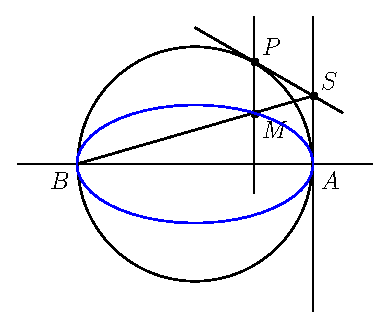
\includegraphics{../images/img005547-1}$$
}
}
